\titre{\tgit}

\begin{quotation}
  \sl Une grande partie de ce TP consiste à lire et comprendre des
  documents sur moodle. Le but n'est pas de le faire le plus
  rapidement possible, mais de comprendre au mieux une architecture
  beaucoup plus complexe que ce que vous avez vu jusque là.
\end{quotation}

\section*{Présentation}

Au cours de ce TP, on va mettre en place les comptes sur différents
sites Web externes qui nous permettront de gérer le code C qui sera
écrit.

\exo{Espace de travail sur Cloud 9}

\question Commencez par ouvrir le mail reçu de \url{support@c9.io} sur
l'adresse mail que vous avez indiqué, et allez sur la page pour créer
un compte.


Un \emph{workspace} (espace de travail) correspond à un projet
unique. Cette définition englobe à la fois les fichiers, les
répertoires, mais aussi un ou plusieurs terminaux, ainsi que la
visualisation de l'ensemble. 

\question Créez un \emph{workspace} appelé \texttt{programmation-c} (tout
en minuscules) comme projet \emph{blank} (icône orange Ubuntu
sur la Fig.~\ref{fig:workspace:creation}).

\begin{figure}[htbp]
  \centering
  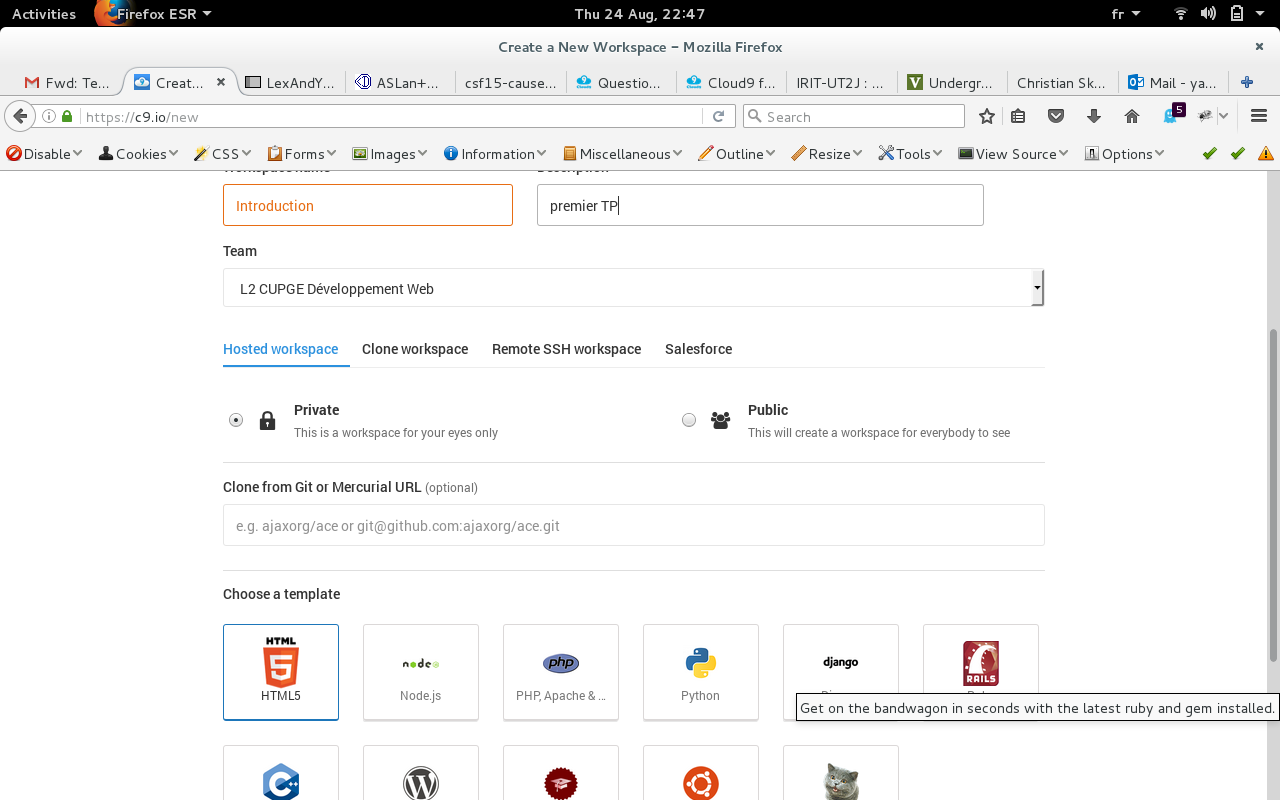
\includegraphics[width=0.9\textwidth]{images/creation_workspace}
  \caption{Fenêtre de création d'un espace de travail.}
  \label{fig:workspace:creation}
\end{figure}

L'environnement de travail ressemble alors à la Fig.~\ref{fig:workspace:initial}.

\begin{figure}[htbp]
  \centering
  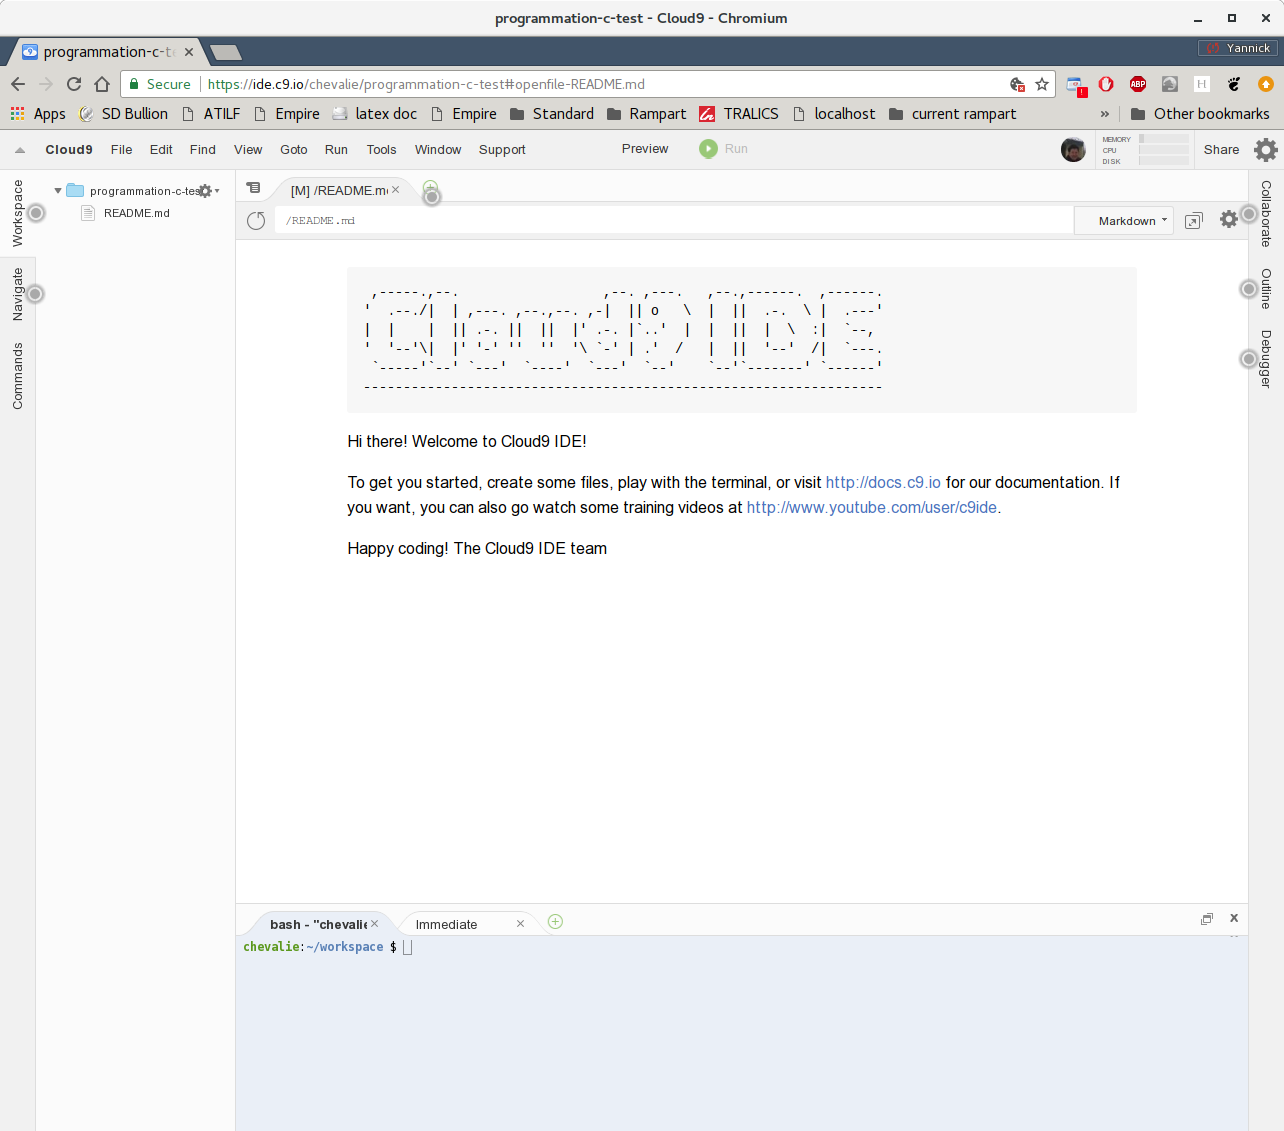
\includegraphics[width=0.9\textwidth]{images/c9_apres_creation.png}
  \caption{Espace de travail intial.}
  \label{fig:workspace:initial}
\end{figure}

\begin{fminipage}{0.9\textwidth}
  Ne fermez pas la fenêtre \url{c9.io}, nous en aurons besoin dans
  l'exercice suivant (il faut ouvrir un nouvel onglet).
\end{fminipage}

\exo{Création d'un compte sur BitBucket}

Pour créer un compte sur \url{https://bitbucket.org/}, il faut
utiliser le lien \texttt{sign up}. Il vous sera demandé une adresse
mail à laquelle sera envoyée un e-mail de confirmation d'inscription.


\question Sur l'écran d'accueil, juste après la validation, cliquez
sur l'icône de profil en bas, à gauche pour accéder à votre tableau de
bord (\emph{dashboard}). Puis allez dans votre compte en cliquant sur
l'icône en bas, à gauche, puis \texttt{view profile},
\texttt{settings}, \texttt{Security}, et \texttt{ssh keys}. On va
relier notre espace de travail sur \url{c9.io} en utilisant la clef
publique ssh créée à l'exercice précédent.

\question Allez ensuite sur \texttt{overview}, et créez un premier
dépôt (repository) (\texttt{Programmation C}, par exemple) comme dépôt
privé. 

\exo{Création d'un site Git sur Cloud 9}

Les données sur Cloud 9 sont correctement sécurisées, mais on veut
pouvoir les exporter facilement, et surtout utiliser un système de
gestion de version, \texttt{git}. Avant de commencez, lisez
l'introduction à git sur moodle. On commence par importer le dépôt
qu'on a crée sur BitBucket:

\begin{solution}
  \begin{bash}{connection:c9:bitbucket}
    cd ~/workspace # normalement inutile
    git clone git@bitbucket.org:NOM/PROJET.git
  \end{bash}
\end{solution}




\exo{Récupérer les énoncés de TP}

Les énoncés de TP sont sur \texttt{\url{http://github.com/}}, un autre site
de gestion de projets.


\question Créez un répertoire vide sur BitBucket.

\question Ajoutez ce répertoire comme répertoire distant pour le
serveur git sur Cloud 9.

\question Mettez à jour le serveur sur BitBucket en fonction de votre
serveur local.  Sur bitbucket, allez dans \texttt{Source} pour
vérifier que tout a bien marché.

\question Éditez le fichier \texttt{README.md} sur C9, sauvegarder (et
``commitez''), et transférer sur BitBucket. Vérifiez que les
transferts marchent correctement.


